\title[Lecture slide retrieval]{Slide retrieval based on lecture recordings}
\mode<presentation>{\subtitle{\color{black}\faGithub\ \href{https://github.com/fi-muni-video-699}{github.com/fi-muni-video-699}}}
\author[V.\,Novotný]{Vít Novotný, witiko@mail.muni.cz}
\year=2018\month=1\day=19
\institute[FI MU]{Faculty of Informatics, Masaryk University}
\subject{Project report}
\keywords{information retrieval, image processing, pattern recognition}

\begin{document}
\begin{frame}[plain]
\maketitle
\end{frame}

\AtBeginSection[]{% Print an outline at the beginning of sections
  \begin{frame}
    \frametitle{Outline for Section~\thesection}
    \begin{multicols}{2}
    \vspace*{-.4em}
    \tableofcontents[currentsection]
    \end{multicols}
  \end{frame}}

\begin{frame}

\mode
<presentation>

\frametitle{Table of contents}
\begin{multicols}{2}
\vspace*{-.4em}

\mode
<all>

\tableofcontents

\mode
<presentation>

\end{multicols}

\mode
<all>

\end{frame}

\mode
<article>


\mode
<all>{%
\section{Introduction}}
Since the spring of 2004, the Faculty of Informatics at the Masaryk University
in Brno, Czech Republic (\abbr{FI} \abbr{MU}) has been recording lectures that
take place in the \abbr{D1}, \abbr{D2}, and \abbr{D3} lecture halls and making
these recordings available to students at the
\href{https://www.video.muni.cz}{video.muni.cz} web site as \term{digital video
files}~\cite{hladkaliska03lectures}. These recordings are a valuable learning
resource; however, due to the lack of information about the structure and the
content of these recordings, it is difficult to
\begin{enumerate}
\item retrieve recordings relevant to the user's \term{information need},
\item find relevant portions in the retrieved recordings, and
\item transform the information contained in the recording to a form that is more
  accessible to visually impaired users.
\end{enumerate}
% As a result, the usefulness of these recordings is rarely fully exploited.

Most lecturers accompany their lectures with \term{lecture slides} that are shown
in the recordings and, at the same time, available to the students as a part of
the course materials in the form of structured \abbr{PDF} documents. One way to
add structured information to the recordings is then to find a mapping between the
temporal dimension of a recording and the pages of the corresponding lecture
slides. This gives us the digital text shown in any given \term{frame} of the
video files, which can be immediately used to
\begin{enumerate}
\item retrieve portions of recordings relevant to the user's information need
  expressed in the form of a text query and
\item convey the text to the visually impaired user using a screen reader, a
  braille display, or another reading device.
\end{enumerate}
Other uses include the improvement of the perceived recording quality by
superimposing a high-resolution rendering of the \abbr{PDF} document pages on
the low-resolution video files.

\mode
<presentation>

\begin{frame}{Introduction}
\begin{itemize}[<+->]
  \item Since 2014, \abbr{FI} \abbr{MU} has been recording lectures in \abbr{D1},
    \abbr{D2}, and \abbr{D3} lecture halls.~\cite{hladkaliska03lectures}
  \item Recordings are available at
    \href{https://www.video.muni.cz}{video.muni.cz}. However, it is difficult to:%
    \begin{enumerate}
      \item retrieve recordings relevant to the user's \term{information need},
      \item find relevant portions in the retrieved recordings, and
      \item transform the recording to a form that is more accessible to visually
        impaired users.
    \end{enumerate}
  \item As a result, the usefulness of these recordings is rarely fully exploited.
  \bigskip
  \item By mapping the temporal dimension of the recordings to lecture
    slides, we can extract the digital text shown in any given frame, which
    can be immediately used to:%
    \begin{enumerate}
      \item retrieve portions of recordings relevant to a text query and
      \item convey the text to the visually impaired user using a reading device.
    \end{enumerate}
  \item Other uses include superimposing a high-resolution rendering of the
    \abbr{PDF} document pages on the low-resolution video files.
\end{itemize}
\end{frame}

\mode
<article>

The text is structured as follows: In Section~\ref{sec:problem}, I will
state the problem, break it down into tasks and describe the evaluation
measures. In Section~\ref{sec:dataset}, I will describe the dataset that I
built for evaluating systems solving the tasks. In
Section~\ref{sec:system-description}, I will describe a baseline system that
solves task 1. In Section~\ref{sec:experimental-setup}, I will describe the
evaluation of the baseline system. In Section~\ref{sec:results}, I will give
the evaluation results. In Section~\ref{sec:conclusion}, I will state my
conclusion. In Section~\ref{sec:future-work}, I will outline venues for future
work.

\mode
<all>{%
\section{Problem statement}
\label{sec:problem}}
In this section, I will describe the problems associated with mapping lecture
recordings to lecture slide pages and specify the tasks a system will need
to~solve.

\mode
<all>{%
\subsection{Sources of noise}
\label{sec:noise}}
To better understand the intricacies of our task, let us first discuss what
kinds of \term{noise} we can expect to appear in our recordings.

\paragraph{Projection} Often, a lecturer will use an unpublished version of the
lecture slides that contains additional pages with \term{incrementally uncovered}
content. In this case, the lecture slides from the course materials may be a
poor match to what is shown on the recordings.

Occasionally, a lecturer will also show their lecture slides in a window rather
than in a full-screen mode. Therefore, finding the position of a projection
screen and finding the position of a lecture slide page within a
\term{projection screen} become two distinct tasks.

Let $\mathcal X$ be the \term{color space} of the lecture slides, $\mathcal Y$
the color space of the \term{projector}, and $\Phi_{\mathcal X},\Phi_{\mathcal
Y}$ the maps to a common color space $\mathbb K$. If the overlap between
$\Phi_{\mathcal X}(\mathcal X)$ and $\Phi_{\mathcal Y}(\mathcal Y)$ is small,
$\Phi^{-1}_{\mathcal Y}(\Phi_{\mathcal X}(\mathcal X))$ will be a poor
representation of $\mathcal X$.

\paragraph{Scene} Even if $\Phi_{\mathcal X}(\mathcal X)\approx\Phi_{\mathcal
Y}(\mathcal Y)$, the \term{reflectance} of the projection screen surface will
distort the colors. Due to the lightning conditions, the projection screen
will in general be \term{unevenly lit}.

\term{Obstacles} positioned between the \term{camera lens} and a projection
screen may partially obscure the recorded lecture slides.

\paragraph{Capture} The guesswork in assessing the \term{color temperature},
the presence of light sources that produce different color spectra compared to
\term{blackbodies}, and the potentially small overlap between $\Phi_{\mathcal
Y}(\mathcal Y)$ and $\Phi_{\mathcal Z}(\mathcal Z)$, where $\mathcal Z$ is the
color space of the camera, will further distort the colors.

Due to the defects in the optical system of the camera, a lecture room
recording will suffer from a number of \term{aberrations} such as defocus and
distortion. In addition, if the camera is not perpendicular to a projection
screen, a \term{perspective transformation} of the recording will be necessary to
\term{crop out} the region corresponding to a projection screen and make it
rectangular. Given an incorrectly positioned camera, or a camera with
\term{telephoto lens}, portions of the projection screen will fall \term{beyond
the bounds} of the captured scene.

Unlike lecture slides, which are generally provided in the form of vector
\abbr{PDF} documents, the resulting digital video files are a result of:
\begin{enumerate}
  \item temporal sampling into frames at a given \term{framerate},
  \item spatial sampling at a given \term{resolution},
  \item light frequency sampling at a given \term{color depth},
  \item \term{chroma subsampling}, and 5. \term{lossy compression}
\end{enumerate}
applied to the original recording. Each of the above reduces the amount of
information present in the digital video file.

\mode
<presentation>

\begin{frame}{Sources of noise I}
\begin{description}[<+->]
  \item[Projection]
    Projected lecture slides may:
    \begin{itemize}
      \item contain additional pages with \term{incrementally uncovered} content,
      \item be shown in a window rather than in a full-screen mode, or
      \item show distorted colors due to small overlap between the color spaces
        of the lecture slides and the projector.
    \end{itemize}

  \item[Scene]
    The \term{reflectance} of a projection screen and uneven illumination
    introduces further noise. 
    \term{Obstacles} positioned between the \term{camera lens} and a projection
    screen may partially obscure the recorded lecture slides.
\end{description}
\end{frame}

\begin{frame}{Sources of noise II}
\begin{description}
\item[Capture]
  Guesswork in assessing \term{color temperature} and small overlap between the
  color spaces of the projector and a camera introduces additional color
  distortion. Defects in the optical system of a camera introduces
  \term{aberrations}.\pause
    
  If the camera is nor perpendicular to a projection screen, a
  \term{perspective transformation} of the recording will be necessary to
  \term{crop out} the projection screen and make it rectangular.
  Given an incorrectly positioned camera, portions of the screen
  will fall \term{beyond the bounds} of the captured scene.\pause

  The resulting digital files are a result of:\pause
  \begin{enumerate}
  \item temporal sampling into frames at a given \term{framerate},\pause
  \item spatial sampling at a given \term{resolution},\pause
  \item light frequency sampling at a given \term{color depth},\pause
  \item \term{chroma subsampling}, and \pause
  \structure{5.} \term{lossy compression} \pause applied to the recording.
  \end{enumerate}
\end{description}
\end{frame}

\mode
<article>


\mode
<all>{%
\subsection{Tasks}
\label{sec:tasks}}
Given the above analysis, a system mapping lecture recordings to lecture slides
will need to solve the following tasks listed in bottom-up order:
\begin{enumerate}
  \item assessing the similarity between a cropped-out projection screen and
    lecture slides, namely
    \begin{enumerate}
      \item mapping a cropped-out projection screen to a lecture slide page, and
      \item deciding if a projection screen matches any lecture slide page,
    \end{enumerate}
  \item detecting and cropping out all projection screens in a single video
    file frame, and
  \item selecting important frames and the order in which frames are resolved.
\end{enumerate}
I will now describe the individual tasks in detail along with the proposed
evaluation method:

\paragraph{Task 1a} Given a single cropped-out projection screen and a set of
lecture slide pages, the task is to retrieve the page in the set that is most
similar to the screen. Since a screen and the matching page may not be
perfectly aligned, rotation~\cite{smith1995simple}, and
translation~\cite{sarvaiyaetal09} coupled with scaling may be necessary to
\term{register} the screen with a page before tackling the noise described in
Section~\ref{sec:noise}.

I will frame this task as an \term{information retrieval} (\abbr{IR}) problem,
i.e.\ I will be looking for an \abbr{IR} system that ranks pages by their
similarity to a screen, so that maching pages receive the highest \term{rank}.
To compare two systems, we can estimate the expected value of the highest
rank of a matching page produced by each system on one or several test
datasets.

\paragraph{Task 1b} Given a single cropped-out projection screen and a set of
lecture slide pages, the task is to decide whether or not the screen matches
any page in the set.\iffalse If a task 1a system produces for each screen not
only a ranking of pages, but also an estimate of distance, similarity, match
confidence, or match probability for each page, and if the random vector of
these estimates can be expected to have a different probability distribution in
the positive case (when a screen matches) and in the negative case, then a
classifier can be trained on one or several training datasets using the
measures produced by a task 1a system as features.\fi

If two systems only produce binary decisions, then we can estimate the expected
values of the \term{misclassification loss} to compare them. If two systems
also report the decision confidence expressed by the distance from a
\term{decision hyperplane}, then we can estimate the expected value of the
\term{binomial deviance}~\cite[sec.~10.6]{friedman2001elements} to compare the
systems. Alternatively, if two systems produce a posterior probability
estimate, then we can estimate the expected values of the
\term{log-likelihood}~\cite[sec.~2.6.3]{friedman2001elements} to compare the
systems.
Informally speaking, both binomial deviance and log-likelihood favor
classifiers that are hesitant about their wrong decisions and confident about
their correct decisions.

\paragraph{Task 2} Given a single video file frame, the task is to detect the
boundaries of all lit projection screens. To compare two systems, we can
estimate the expected value of the \term{Jaccard index} between each system and
one or several test datasets using polygonal union and intersection.

\paragraph{Task 3} Given a single recording, the task is to detect the frames
at which the following events take place:
\begin{enumerate}
  \item a new projection screen is lit,
  \item a projection screen is no longer lit, or
  \item a projection screen shows new content.
\end{enumerate}
To compare two systems, we can take events of each type and estimate the
expected value of a segmentation similarity metric such as boundary similarity
($\textrm B$)~\cite{P13-1167} for an event type between each system on one or
several test datasets.

\mode
<presentation>

\begin{frame}{Tasks}
\begin{description}[<+->]
  \item[Task 1a]
    Given a single cropped-out projection screen and a set of lecture slide
    pages, the task is to retrieve the page that is most similar to the screen.

  \item[Task 1b]
    Given a single cropped-out projection screen and a set of lecture slide
    pages, the task is to decide whether the screen matches any page in the set.

  \item[Task 2]
    Given a single video file frame, the task is to detect the boundaries of all
    lit projection screens.

  \item[Task 3]
    Given a single recording, the task is to detect the frames at which the
    following events take place:
    \begin{enumerate}
      \item a new projection screen is lit,
      \item a projection screen is no longer lit, or
      \item a projection screen shows new content.
    \end{enumerate}
\end{description}
\end{frame}

\mode
<article>


\mode
<all>{%
\section{Dataset}
\label{sec:dataset}}
As a first step in building and evaluating a system solving the above tasks, I
built a dataset from the recordings published at
\href{https://www.video.muni.cz}{video.muni.cz}.
Although the recordings date as far back as 2004, I restricted myself to the
recordings from the \abbr{D1}, \abbr{D2}, and \abbr{D3} lecture halls taken
during 2010--2016. This was mainly due to the difficulty in reaching out to
the lecturers who are often no longer a part of the faculty, and the variance
in the video file format encoding and resolution. From the uniform distribution
of these recordings, I drew a random sample that would form my dataset.

The original sample consisted of 20 recordings. For three recordings, I was
unable to establish communication with the lecturers to request their consent.
For three other recordings, the lecturers would not give consent to including
the recordings in the dataset; I drew three recordings from the uniform
distribution of recordings as substitutes.
The dataset has been published in a Git repository.\footnote{See
  \href{https://github.com/fi-muni-video-699/dataset}%
       {github.com/fi-muni-video-699/dataset} or
  \href{https://gitlab.fi.muni.cz/xnovot32/fi-muni-video-699}%
       {gitlab.fi.muni.cz/xnovot32/fi-muni-video-699}.}

\mode
<all>{%
\subsection{Dataset structure}}
The dataset consists of 17 recordings. For the purpose of solving tasks 1 and
2, a recording consists of a set of lecture slides and a sample of the video
file frames. Since the systems solving tasks 1 and 2 will only be invoked by
the system solving task 3 when one of the events described in
Section~\ref{sec:tasks} takes place, I did not assume uniform distribution of
the frames when drawing a sample. Instead, I reduced each uneventful segment of
the recording into a single frame by drawing from the uniform distribution of
frames forming the segment. A random sample of up to 25 frames was then drawn
from the uniform distribution of the reduced segments. For each frame in the
sample, I marked the boundaries of all lit screens and described the pages of
the lecture slides shown on the screens.

The dataset is represented by an \abbr{XML} document \texttt{dataset.xml} in
the language \texttt{schema.xsd} shown in Figure~\ref{fig:schema}. The root
element of \texttt{dataset.xml} consists of a sequence of recordings
represented by video elements. I will now describe the individual elements of
the language:

\mode
<presentation>

\begin{frame}{Dataset structure I}
The dataset consists of 17 recordings. It is represented by an \abbr{XML}
document \texttt{dataset.xml} in the language \texttt{schema.xsd}:
\begin{center}
  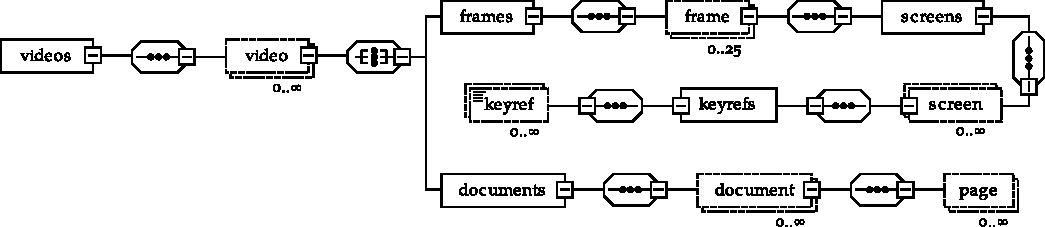
\includegraphics[width=\textwidth]{fig/structure/schema}
\end{center}
\end{frame}

\mode
<article>

\begin{figure}
  \leavevmode\kern-0.13\textwidth
  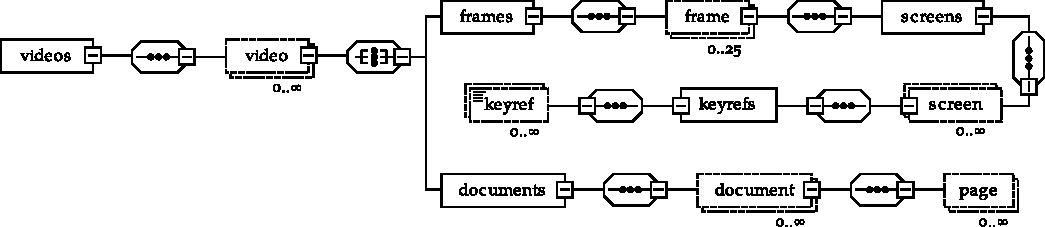
\includegraphics[width=1.4\textwidth]{fig/structure/schema}
  \caption{The \abbr{XML} language \texttt{schema.xsd} \iffalse produced using the
    \term{\abbr{XSD} diagram} tool\fi}
  \label{fig:schema}
\end{figure}

\subsubsection*{The video element}
A video element corresponds to a single lecture recording and contains the
following attributes:
\begin{description}
  \item[dirname] the name of the directory containing the frames and lecture slides,
  \item[uri] an \abbr{URI} of the video file containing the recording,
  \item[fps] the framerate of the video file,
  \item[frames] the length of the video file in frames, and
  \item[width\textmd, height] the resolution of the video file.
\end{description}
Beside the attributes, a video element contains a sequence of video file frames
and lecture slides represented by frame elements and document elements,
respectively.

\subsubsection*{The frame element}
A frame element corresponds to a single frame of a video file and contains the
following attributes:
\begin{description}
  \item[number] the frame number in the video file,
  \item[vgg256] two \term{\abbr{vgg} feature vectors} obtained by feeding the
    entire frame into two 256dimensional \term{\abbr{VGG} convolutional neural
    networks}~\cite{simonyan2014very} -- the first trained on the ImageNet%
    \note{See \href{http://www.image-net.org/}{image-net.org}.} image
    classification dataset and the second trained on the ImageNet and
    Places2\note{See \href{http://places2.csail.mit.edu/}{places2.csail.mit.edu}.}
    datasets -- and taking the last hidden layer, and
  \item[filename] the filename of the image file containing the frame.
\end{description}
Beside the attributes, a frame element contains a sequence of lit projection
screens represented by screen elements.

\subsubsection*{The screen element}
A screen element corresponds to a single lit projection screen on a single
frame of a video file and contains the following attributes:
\begin{description}
  \item[x0\textmd, y0\textmd, x1\textmd, y1\textmd, x2\textmd, y2\textmd,
        x3\textmd, y3] coordinates with respect to the current frame
    of the recording that specify the four corners of a quadrilinear
    bounding a single lit projection screen,
  \item[condition] the types of noise affecting this video file frame:
    \begin{description}
      \item[windowed] the projection screen shows a lecture slide in a window
        rather than in a full-screen mode,
      \item[obstacle] an obstacle positioned between the camera lens and the
        projection screen partially obscures the lecture slide, and
      \item[pristine] none of the above, and
    \end{description}
  \item[vgg256] two \abbr{VGG} feature vectors obtained by feeding the
    cropped-out projection screen into the neural networks described in
    the section about the frame element.
\end{description}
Beside the attributes, a screen element is in a relation to pages of lecture
slides that is represented by a sequence of keyref elements.

\afterpage{%
\begin{landscape}
\begin{figure}
  \leavevmode\kern-.117\paperheight
  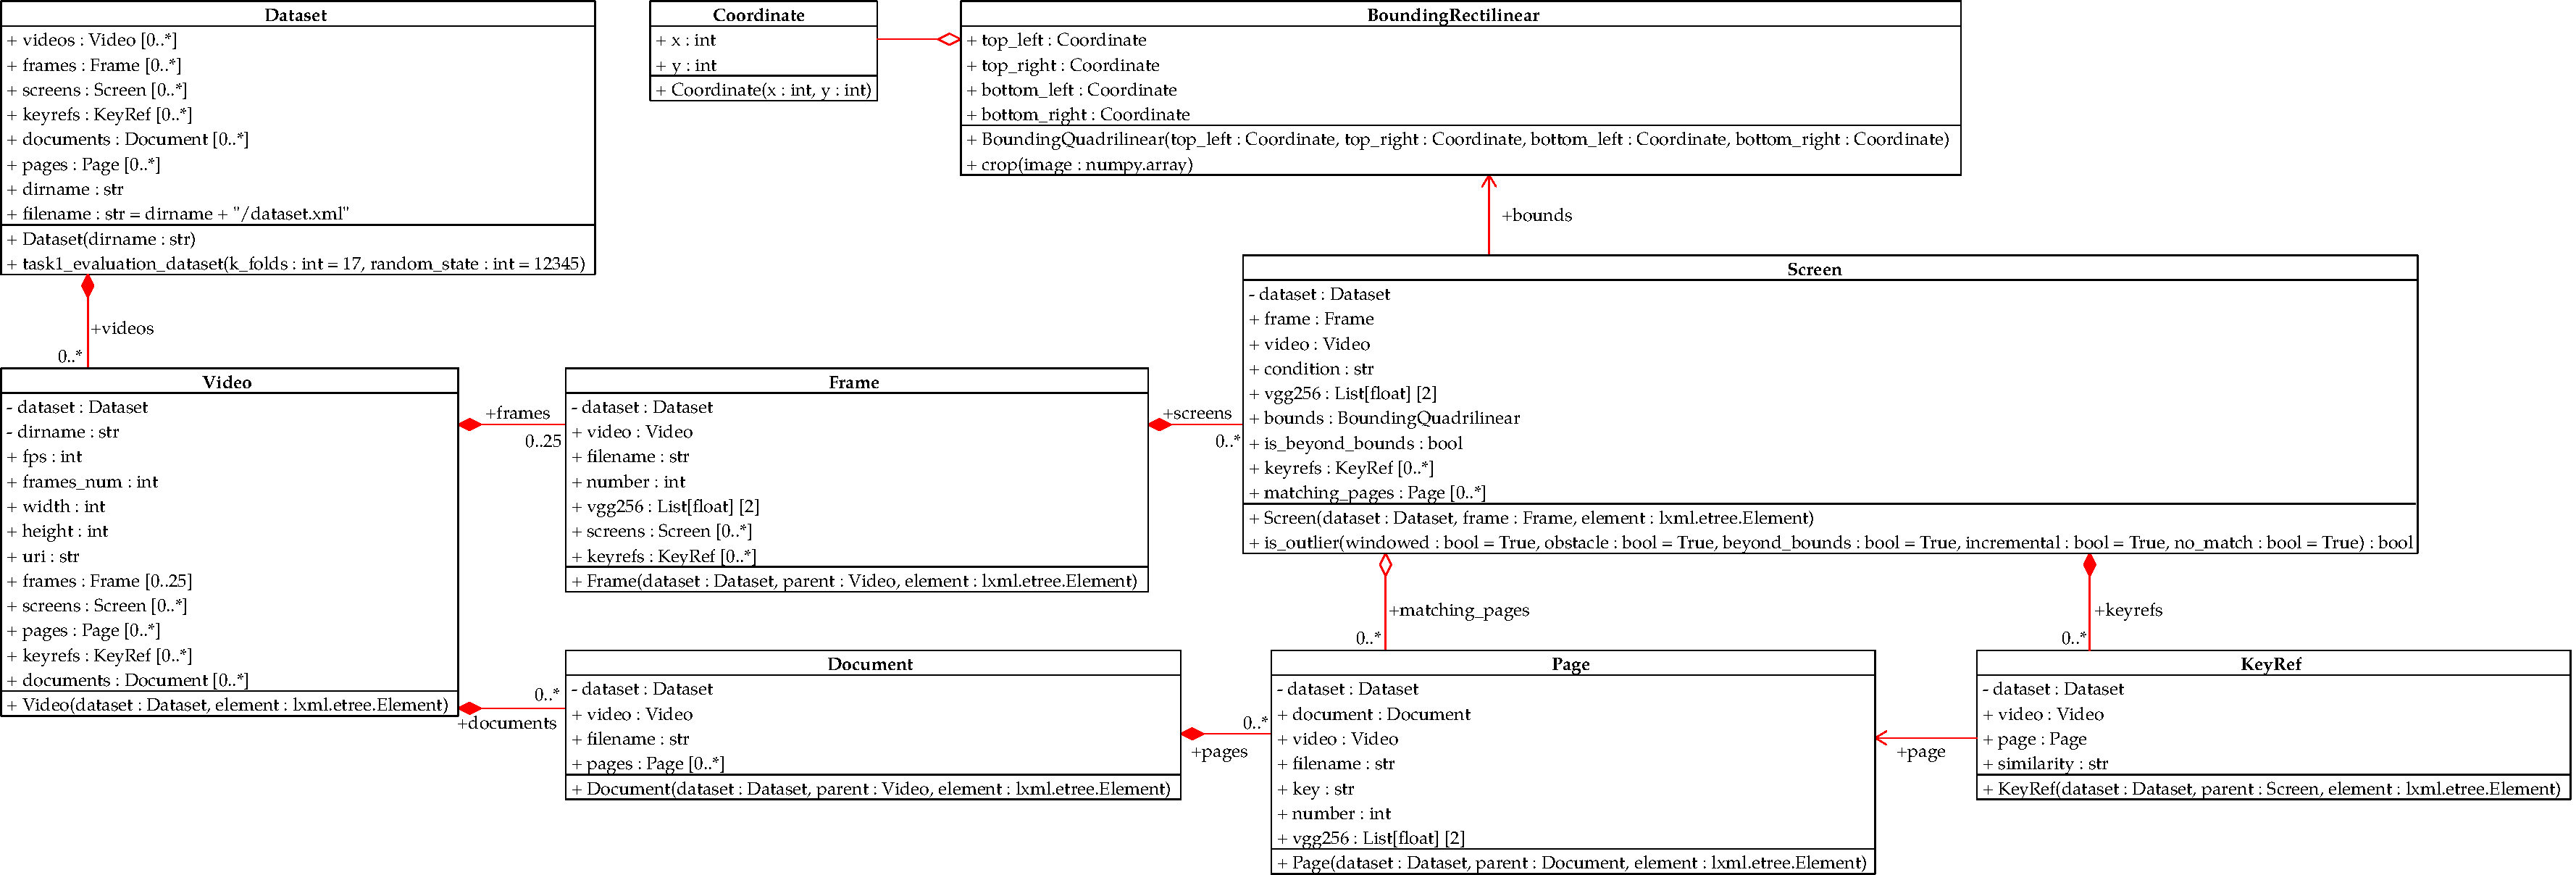
\includegraphics[width=.95\paperheight]{fig/structure/uml}
  \caption{A \abbr{UML} class diagram of the Python interface for the dataset
    \iffalse produced using the \term{Umbrello} tool\fi}
  \label{fig:uml}
\end{figure}
\end{landscape}}

\subsubsection*{The keyref element}
A keyref element corresponds to a single 2-tuple from a binary relation between
lit projection screens and lecture slide pages and contains the following
attribute:
\begin{description}
  \item[similarity] the type of relation between this lit projection screen and
    a lecture slide page:
    \begin{description}
      \item[full] the projection screen $s$ shows the lecture slide page $p$
        ($s\approx p$), and
      \item[incremental] a single \term{logical} lecture slide page is split
        across several lecture slide pages and incrementally uncovered; the
        projection screen $s$ and the lecture slide page $p$ correspond to the
        same logical page ($s\sim p$).
    \end{description}
\end{description}
Beside the attribute, a keyref element contains a reference to a lecture slide
page represented the unique identifier of a page element.

During the task description in Section~\ref{sec:tasks}, I talked somewhat
vaguely about a projection screen „matching“ a lecture slide page. To give a
precise definition, a lit projection screen $s$ matches a lecture slide page $p$ if
and only if \[s\approx p\lor\big(\nexists p'(s\approx p')\land s\sim p\big).\]

\subsubsection*{The document element}
A document element corresponds to a single set of lecture slides and contains
the following attribute:
\begin{description}
  \item[filename] the filename of the \abbr{PDF} file containing the lecture slides.
\end{description}
Beside the attribute, a document element contains a sequence of lecture slide
pages screens represented by page elements.

\subsubsection*{The page element}
Each page element corresponds to a single page of lecture slides and contains
the following attribute:
\begin{description}
  \item[key] a identifier of the page that is unique in the current video element,
  \item[filename] the filename of the image file containing the page,
  \item[number] the number of the page in the \abbr{PDF} document,
  \item[vgg256] two \abbr{VGG} feature vectors obtained by feeding the page
    into the neural networks described in the section about the frame element.
\end{description}

\mode
<all>

\begin{frame}[fragile]
\frametitle<presentation>{Dataset structure II}
\mode<article>{%
The dataset is distributed along with a Python interface implemented in files
\texttt{dataset.py} and \texttt{review.py} whose class diagram is shown in
Figure~\ref{fig:uml}. Load the dataset as follows:}
\mode<presentation>{%
The dataset is distributed along with a Python interface. Load it as follows:}
\begin{listings}
\begin{minted}{bash}
$ git clone https://github.com/fi-muni-video-699/dataset.git
$ mkvirtualenv -p $(which python3) dataset
(dataset) $ pip install -U pip; pip install -r dataset/requirements.txt
(dataset) $ python
\end{minted}
\begin{minted}{python}
>>> import logging; from dataset import Dataset
>>> logging.basicConfig(level=logging.INFO, format="%(message)s")
>>> dataset = Dataset("dataset")
\end{minted}
\begin{verbatim}
Validating the dataset …
Done validating the dataset.
Processing the dataset …
Done processing the dataset, which contains:
- 17 videos containing 409 frames with 683 screens (93 non-matched)
  and 699 keyrefs, and
- 25 documents containing 925 pages.
\end{verbatim}
\end{listings}
\end{frame}

\mode
<article>


\mode
<all>{%
\subsection{Examples}
\label{sec:examples}}
To give a better sense of the structure of the dataset, I will now give several
examples along with the corresponding \abbr{XML} code, and the images of the
video file frames, projection screens, and lecture side pages. I sorted the
individual structures in an increasing order of rarity. Examples are shown in
figures \ref{fig:example-first}--\ref{fig:example-last}.

\begin{description}
  \begin{figure}
    \inputminted{xml}{fig/examples/normal/example.xml}\par
    \showthreeimages{fig/examples/normal}%
      {frame006000.png}{frame006000-00.png}{slides01-30.png}%
      {The image file \texttt{frame006000.png}}%
      {A cropped-out \texttt{frame006000.png}}%
      {The image file \texttt{slides01-30.png}}
    \caption{A screen element in the usual case. Both the abbreviated code
      of the \texttt{dataset.xml} document (above) and the video file frame,
      cropped-out projection screen, and the lecture slide page (below) are
      shown.}
    \label{fig:example-normal}
    \label{fig:example-first}
  \end{figure}
  \item[The usual case] In 371 out of the total 683 screen elements, the
    projection screen is captured fully without any obstacles positioned
    between the camera lens and the screen and it shows a single page from the
    associated lecture slides in full-screen mode. An example is shown in
    Figure~\ref{fig:example-normal}.

\mode
<presentation>

  \begin{frame}{The usual case}
    In 371 out of the total 683 screen elements, the projection screen is
    captured fully without any obstacles positioned between the camera lens and
    the screen and it shows a single page from the associated lecture slides in
    full-screen mode:

    \showthreeimages{fig/examples/normal}%
      {frame006000.png}{frame006000-00.png}{slides01-30.png}
  \end{frame}

\mode
<article>

  \begin{figure}
    \inputminted{xml}{fig/examples/incremental/example.xml}\par
    \showtwoimages{fig/examples/incremental}%
      {frame052000.png}{frame052000-01.png}%
      {The image file \texttt{frame052000.png}}%
      {A cropped-out \texttt{frame052000.png}}\par
    \showthreeimages{fig/examples/incremental}%
      {slides01-31.png}{slides01-32.png}{slides01-33.png}%
      {The image file \texttt{slides01-31.png}}%
      {The image file \texttt{slides01-32.png}}%
      {The image file \texttt{slides01-33.png}}
    \caption{A screen element with incrementally matching lecture slides.}
    \label{fig:example-incremental}
  \end{figure}
  \item[Incremental matches] In 125 out of the total 683 screen elements,
    the projection screen shows only the same logical page as some of the
    lecture slide pages. An example is shown in
    Figure~\ref{fig:example-incremental}.

\mode
<presentation>

  \begin{frame}{Incremental matches}
    In 125 out of the total 683 screen elements,
    the projection screen shows only the same logical page as some of the
    lecture slide pages:

    \showtwoimages{fig/examples/incremental}%
      {frame052000.png}{frame052000-01.png}%
  \end{frame}
  \begin{frame}[plain]
    \showtwoimages{fig/examples/incremental}%
      {frame052000.png}{frame052000-01.png}%
    \showthreeimages{fig/examples/incremental}%
      {slides01-31.png}{slides01-32.png}{slides01-33.png}%
  \end{frame}

\mode
<article>

  \begin{figure}
    \inputminted{xml}{fig/examples/beyond-bounds/example.xml}\par
    \showthreeimages{fig/examples/beyond-bounds}%
      {frame004000.png}{frame004000-00.png}{slides01-12.png}%
      {The image file \texttt{frame004000.png}}%
      {A cropped-out \texttt{frame004000.png}}%
      {The image file \texttt{slides01-12.png}}
    \caption{A screen element that extends beyond the bounds of the recording.}
    \label{fig:example-beyond-bounds}

    \kern\floatsep
    \inputminted{xml}{fig/examples/no-keyrefs/example.xml}\par
    \showthreeimages{fig/examples/no-keyrefs}%
      {frame004000.png}{frame004000-00.png}{frame004000-01.png}%
      {The image file \texttt{frame004000.png}}%
      {A cropped-out \texttt{frame004000.png}}%
      {A cropped-out \texttt{frame004000.png}}
    \caption{Two screen elements with no matching lecture slide pages.}
    \label{fig:example-no-keyrefs}
  \end{figure}
  \item[A screen beyond bounds] In 108 out of the total 683 screen elements,
    the projection screen is captured only partially in the recording.
    An example is shown in Figure~\ref{fig:example-beyond-bounds}.
  \item[No matching pages] In 93 out of the total 683 screen elements, the
    projection screen shows none of the lecture slide pages – a condition
    that a system solving task 1b should be able to detect.
    An example is shown in Figure~\ref{fig:example-no-keyrefs}.

\mode
<presentation>

  \begin{frame}{A screen beyond bounds}
    In 108 out of the total 683 screen elements, the projection screen is
    captured only partially in the recording:

    \showthreeimages{fig/examples/beyond-bounds}%
      {frame004000.png}{frame004000-00.png}{slides01-12.png}%
  \end{frame}
  \begin{frame}{No matching pages}
    In 93 out of the total 683 screen elements, the projection screen shows
    none of the lecture slide pages – a condition that a system solving task 1b
    should be able to detect:

    \showthreeimages{fig/examples/no-keyrefs}%
      {frame004000.png}{frame004000-00.png}{frame004000-01.png}%
  \end{frame}

\mode
<article>

  \begin{figure}
    \inputminted{xml}{fig/examples/incremental-only/example.xml}\par
    \showthreeimages{fig/examples/incremental-only}%
      {frame040000.png}{frame040000-00.png}{slides02-06.png}%
      {The image file \texttt{frame040000.png}}%
      {A cropped-out \texttt{frame0040000.png}}%
      {The image file \texttt{slides02-06.png}}
    \caption{A screen element with only incrementally matching lecture slides.}
    \label{fig:example-incremental-only}

    \kern\floatsep
    \inputminted{xml}{fig/examples/windowed/example.xml}\par
    \showthreeimages{fig/examples/windowed}%
      {frame080000.png}{frame080000-01.png}{slides01-02.png}%
      {The image file \texttt{frame080000.png}}%
      {A cropped-out \texttt{frame080000.png}}%
      {The image file \texttt{slides01-02.png}}
    \caption{A screen element showing a lecture slide page in a window rather
      than in a full-screen mode.}
    \label{fig:example-windowed}
  \end{figure}
  \item[Only incremental matches] In 60 out of the total 683 screen elements,
    the projection screen shows none of the lecture slide pages; it shows only
    the same logical page as some of the lecture slide pages.
    An example is shown in Figure~\ref{fig:example-incremental-only}.
  \item[A windowed lecture slide] In 6 out of the total 683 screen elements,
    the projection screen shows a lecture slide page in a window rather than
    in a full-screen mode. An example is shown in
    Figure~\ref{fig:example-windowed}.

\mode
<presentation>

  \begin{frame}{Only incremental matches}
    In 60 out of the total 683 screen elements, the projection screen shows
    none of the lecture slide pages; it shows only the same logical page as
    some lecture slide page:

    \showthreeimages{fig/examples/incremental-only}%
      {frame040000.png}{frame040000-00.png}{slides02-06.png}%
  \end{frame}
  \begin{frame}{A windowed lecture slide}
    In 6 out of the total 683 screen elements,
    the projection screen shows a lecture slide page in a window rather than
    in a full-screen mode:

    \showthreeimages{fig/examples/windowed}%
      {frame080000.png}{frame080000-01.png}{slides01-02.png}%
  \end{frame}

\mode
<article>

  \begin{figure}[!t]
    \inputminted{xml}{fig/examples/obstacle/example.xml}\par
    \showthreeimages{fig/examples/obstacle}%
      {frame090000.png}{frame090000-01.png}{slides01-28.png}%
      {The image file \texttt{frame090000.png}}%
      {A cropped-out \texttt{frame090000.png}}%
      {The image file \texttt{slides01-28.png}}
    \caption{A screen element obscured by an obstacle (a blackboard) positioned
      between the camera lens and the projection screen.}
    \label{fig:example-obstacle}
    \label{fig:example-last}
  \end{figure}
  \item[Obscured projection screen] In 5 out of the total 683 screen elements,
    the projection screen is partially obscured by an obstacle positioned
    between the camera lens and the screen.
    An example is shown in Figure~\ref{fig:example-obstacle}.

\mode
<presentation>

  \begin{frame}{Obscured projection screen}
    In 5 out of the total 683 screen elements,
    the projection screen is partially obscured by an obstacle positioned
    between the camera lens and the screen:

    \showthreeimages{fig/examples/obstacle}%
      {frame090000.png}{frame090000-01.png}{slides01-28.png}%
  \end{frame}

\mode
<article>
\end{description}

\FloatBarrier
\mode
<all>{%
\section{System description}
\label{sec:system-description}}
To provide a baseline for future systems and a reference for using the Python
interface for the dataset, I implemented a baseline system that solves task 1.
In this section, I will give a description of its structure and the used
techniques.  An implementation of the system has been published in a Git
repository.\footnote{See
  \href{https://github.com/fi-muni-video-699/system}%
       {github.com/fi-muni-video-699/system} or
  \href{https://gitlab.fi.muni.cz/xnovot32/fi-muni-video-system}%
       {gitlab.fi.muni.cz/xnovot32/fi-muni-video-system}.}

\mode
<all>{%
\subsection{Preprocessing}
\label{sec:preprocessing}}
The video frame images and lecture slide page images are preprocessed in the
\texttt{preprocessing.Image.get\_image} method. I will now describe the
individual steps in order of execution. Examples are shown in figures~%
\ref{fig:preprocessing-first}--\ref{fig:preprocessing-last}.

\begin{figure}
  \showthreeimages{fig/preprocessing}%
    {page_rgb}{frame_rgb}{other_frame_rgb}%
    {The image file \texttt{slides01-04.png} ($I_1$)}%
    {The image file \texttt{frame004000.png} ($I'_2$)}%
    {The image file \texttt{frame050000.png} ($I'_3$)}\par
  \showtwoimages{fig/preprocessing}%
    {screen_rgb}{other_screen_rgb}%
    {A cropped-out \texttt{frame004000.png} ($I_2$)}%
    {A cropped-out \texttt{frame050000.png} ($I_3$)}
  \caption{Cropping out a screen from two different video frame images, one
    matching the given lecture slide page and the other one not.}
  \label{fig:preprocessing-first}

  \kern\floatsep
  \showthreeimages{fig/preprocessing}%
    {page_img_noillumination}{screen_img_noillumination}{other_screen_img_noillumination}%
    {The relative luminance of $I_1$ ($Y_1$)}%
    {The relative luminance of $I_2$ ($Y'_2$)}%
    {The relative luminance of $I_3$ ($Y'_3$)}
  \caption{Color removal and relative luminance flipping in images $I_1,
    I_2$, and~$I_3$.}
\end{figure}
\begin{description}
  \item[Cropping out a screen]
    Since the system does not solve task 2, it expects to be given the
    boundaries of a lit projection screen along with a video frame image. By
    applying a perspective transform~\cite[sec.~2]{eberly11}, I crop out the
    projection screen out of the frame image.
  \item[Color removal]
    As noted in Section~\ref{sec:noise}, I expect a significant mismatch
    between the colors in a cropped-out projection screen image and the colors
    in a lecture slide page image. Although the hue differs arbitrarily, I
    assume that if we disregard uneven illumination, the \term{relative
    luminance} in the cropped-out projection screen image is an affine
    transformation of the relative luminance in the corresponding lecture slide
    page image. Therefore, I reduce an image $I$ to the relative luminance
    $Y=0.2126\cdot R+0.7152\cdot G+0.0722\cdot B$~\cite[part~2]{stokesetal96},
    where $R,G$, and $B$ are the red, green, and blue channels of $I$ expressed
    in the linear \abbr{RGB} color space.
  \item[Relative luminance flipping]
    I assume that each lecture slide page can be conceptually broken down into
    a foreground containing text and figures, and a background.
    More formally stated, I assume that if we disregard uneven illumination,
    the relative luminance $Y$ of a lecture slide page image pixel can be
    accurately modeled as a continuous bivariate random variable with. Under
    this model, the system needs to first decide whether the foreground is
    brighter or darker compared to the background.
    
    Given the observation that the background is typically significantly
    larger that the foreground, I use the Otsu's
    method~\cite{otsu1979threshold} to threshold~$Y$. If the ratio between the
    number of pixels above and below the threshold is greater than $1.8$, I
    assume that the foreground is darker than the background. Otherwise, I
    \term{flip} the relative luminance and assign $Y\leftarrow1-Y$.
    Optionally, this step may be skipped; this choise is controlled by the
    parameter $\theta_1$.

\mode
<presentation>

  \begin{frame}{Cropping out a screen}
    Since the system does not solve task 2, it expects to be given the
    boundaries of a lit projection screen along with a video frame image. By
    applying a perspective transform~\cite[sec.~2]{eberly11}, I crop out the
    projection screen out of the frame image:

    \showthreeimages{fig/preprocessing}%
      {page_rgb}{frame_rgb}{other_frame_rgb}%
  \end{frame}
  \begin{frame}[plain]
    \showthreeimages{fig/preprocessing}%
      {page_rgb}{frame_rgb}{other_frame_rgb}%
    \showtwoimages{fig/preprocessing}%
      {screen_rgb}{other_screen_rgb}%
  \end{frame}

  \begin{frame}{Color removal and relative luminance flipping}
    I reduce an image $I$ to the relative luminance $Y=0.2126\cdot
    R+0.7152\cdot G+0.0722\cdot B$.\pause

    Since the background is typically significantly larger that the foreground,
    I use the Otsu's method~\cite{otsu1979threshold} to threshold~$Y$. If the
    ratio between the number of pixels above and below the threshold is less
    than $1.8$, I \term{flip} the relative luminance and assign
    $Y\leftarrow1-Y$:

  \showthreeimages{fig/preprocessing}%
    {page_img_noillumination}{screen_img_noillumination}{other_screen_img_noillumination}%
  \end{frame}

\mode
<article>

  \begin{figure}
    \showtwoimages{fig/preprocessing}%
      {J}{J_}%
      {The morphological closing $\gamma_\blacksquare(Y'_2)$}%
      {The morphological closing $\gamma_\blacksquare(Y'_3)$}\par
    \showthreeimages{fig/preprocessing}%
      {page_img_noillumination}{screen_img}{other_screen_img}%
      {The relative luminance of $I_1$ ($Y_1$)}%
      {Evenly illuminated $Y'_2$ ($Y_2$)}%
      {Evenly illuminated $Y'_3$ ($Y_3$)}
    \caption{Uneven illumination removal, intensity stretching, and change of
      size in images $I_1,I_2$, and $I_3$ with a rectangular structuring
      element of size $\theta_2 = 65$.}

    \kern\floatsep
    \showthreeimages{fig/preprocessing}%
      {page_img-bw}{screen_img-bw}{other_screen_img-bw}%
      {The foreground of $I_1$ ($F_1$)}%
      {The foreground of $I_2$ ($F_2$)}%
      {The foreground of $I_3$ ($F_3$)}
    \caption{Binarization of images $I_1,I_2$, and $I_3$.}
    \label{fig:preprocessing-last}
  \end{figure}
  \item[Uneven illumination removal]
    To remove the uneven illumination in a cropped-out presentation screen
    image, I first fill the holes (i.e.\ the foreground pixels) in $Y$ by
    applying a \term{morphological closing} $\gamma_\blacksquare$ with a
    rectangular \term{structural element} of size $\theta_2$, where
    $\theta_2\in\{2^i+1\mid i=0,1,\ldots,\log_2 512\}$
    is a parameter, and with the assumption that pixels beyond the image
    boundaries have the value $\infty$ for \term{morphological erosion} and
    $-\infty$ for \term{morphological dilation}. I then assign $Y\leftarrow
    1-(\gamma_\blacksquare(Y)-Y)$.  This way, only the depth of the holes is retained and
    not their difference in elevation caused by uneven illumination.
  \item[Intensity stretching]
    As stated above, I assume that the \term{relative luminance} in the
    cropped-out projection screen image is an affine transformation of the
    relative luminance in the corresponding lecture slide page image. To make
    the relative luminance of the two images identical, I perform a
    \term{linear stretching} of $Y$ and assign
    $Y\leftarrow\frac{Y-\min(Y)}{\max(Y)-\min(Y)}$.
  \item[Change of size]
    To work with homogeneous data, I resize all images to the resolution of
    $512\times 512$ pixels.
  \item[Binarization]
    As stated above, I assume that each lecture slide page can be broken down
    into a foreground, and a background. For each image, I use
    the Otsu's method~\cite{otsu1979threshold} to threshold~$Y$ into dark
    foreground pixels $F$. $F$ is then denoised by applying a
    \term{morphological opening by reconstruction} with an elliptical
    structural element of size 3, and by removing any connected regions
    touching the image boundary.

\mode
<presentation>

  \begin{frame}{Uneven illumination removal, intensity stretching, change of size}
    To remove the uneven illumination in a cropped-out presentation screen
    image, I use \term{morphological closing} $\gamma_\blacksquare$. I assign
    $Y\leftarrow 1-(\gamma_\blacksquare(Y)-Y)$.\pause

    To make the relative luminance of the two images identical, I assign
    $Y\leftarrow\frac{Y-\min(Y)}{\max(Y)-\min(Y)}$.\pause

    To work with homogeneous data, I resize all images to the resolution of
    $512\times 512$ pixels:

    \showthreeimages{fig/preprocessing}%
      {page_img_noillumination}{screen_img}{other_screen_img}%
  \end{frame}
  \begin{frame}[plain]
    \showtwoimages{fig/preprocessing}%
      {J}{J_}%
    \showthreeimages{fig/preprocessing}%
      {page_img_noillumination}{screen_img}{other_screen_img}%
  \end{frame}

  \begin{frame}{Binarization}
    For each image, I use the Otsu's method~\cite{otsu1979threshold} to
    threshold~$Y$ into dark foreground pixels $F$. $F$ is denoised by
    applying a \term{morphological opening by reconstruction} with an
    elliptical structural element of size 3, and by removing regions touching
    the image boundary:

    \showthreeimages{fig/preprocessing}%
      {page_img-bw}{screen_img-bw}{other_screen_img-bw}%
  \end{frame}

\mode
<article>
\end{description}

\mode
<all>{%
\subsection{Feature extraction}
\label{sec:features}}
After processing an image, descriptors are extracted from the
relative luminance $Y$ and the foreground $F$. I will now describe the
\term{features} recognized by the~system:

\begin{description}
  \item[Haralick features]
    52 Haralick texture features~\cite{haralick1973textural} are extracted from $Y$.

  \begin{figure}
    \showthreeimages{fig/preprocessing}%
      {page_img-rows}{screen_img-rows}{other_screen_img-rows}%
      {The morphological dilation $\delta_{{}-{}}(F_1)$}%
      {The morphological dilation $\delta_{{}-{}}(F_2)$}%
      {The morphological dilation $\delta_{{}-{}}(F_3)$}
    \caption{Foreground rows of images $I_1,I_2$, and $I_3$.}
    \label{fig:system-features-rows}

    \kern\floatsep
    {\setlength{\fboxrule}{0pt}%
     \showthreeimages{fig/preprocessing}%
       {row_histogram-0_0}{row_histogram-0_1}{row_histogram-0_2}%
       {The histogram of $I_1$'s row heights}%
       {The histogram of $I_2$'s row heights}%
       {The histogram of $I_3$'s row heights}\par
     \showthreeimages{fig/preprocessing}%
       {row_histogram-1_0}{row_histogram-1_1}{row_histogram-1_2}%
       {The histogram of $I_1$'s row altitudes}%
       {The histogram of $I_2$'s row altitudes}%
       {The histogram of $I_3$'s row altitudes}}
    \caption{Foreground row histograms of images $I_1,I_2$, and $I_3$.}
    \label{fig:system-features-row-histograms}
  \end{figure}
  \item[Foreground rows]
    Rows are extracted from $F$ by applying morphological dilation $\delta_{{}-{}}$ with
    a structural element in the shape of a horizontal line of length $2\times
    512+1$. An example is shown in Figure~\ref{fig:system-features-rows}.
    To obtain a fixed number of features, the row heights and altitudes are each
    represented by a histogram with 16 equal-width bins. An example is shown in
    Figure~\ref{fig:system-features-row-histograms}. Combined with the number
    of rows, this yields 33 features.

\mode
<presentation>

  \begin{frame}{Foreground rows I}
    Rows are extracted from $F$ by applying morphological dilation
    $\delta_{{}-{}}$ with a structural element in the shape of a horizontal
    line of length $2\times 512+1$:

    \showthreeimages{fig/preprocessing}%
      {page_img-rows}{screen_img-rows}{other_screen_img-rows}%
  \end{frame}
  \begin{frame}{Foreground rows II}
    To obtain a fixed number of features, the row heights are represented by a
    histogram with 16 equal-width bins:

    {\setlength{\fboxrule}{0pt}%
     \showthreeimages{fig/preprocessing}%
       {row_histogram-0_0}{row_histogram-0_1}{row_histogram-0_2}}
  \end{frame}
  \begin{frame}{Foreground rows III}
    To obtain a fixed number of features, the row altitudes are represented by
    a histogram with 16 equal-width bins:

    {\setlength{\fboxrule}{0pt}%
     \showthreeimages{fig/preprocessing}%
       {row_histogram-1_0}{row_histogram-1_1}{row_histogram-1_2}}
  \end{frame}

\mode
<article>

  \begin{figure}
    {\setlength{\fboxrule}{0pt}%
     \showthreeimages{fig/preprocessing}%
       {histogram-1_0}{histogram-1_1}{histogram-1_2}%
       {The histogram of $\delta_{{}-{}}(F_1)\cdot Y_1$}%
       {The histogram of $\delta_{{}-{}}(F_2)\cdot Y_2$}%
       {The histogram of $\delta_{{}-{}}(F_3)\cdot Y_3$}}
    \caption{Relative luminance histograms of images $I_1,I_2$, and $I_3$ computed from
      the foreground row pixels.}
    \label{fig:system-features-relative-luminance}
  \end{figure}
  \item[Relative luminance]
    A histogram is extracted from $Y$ with 16 equal-width bins. Optionally, the
    histogram can be extracted only from foreground row pixels and each pixel
    can be assigned a weight according to its variance across all lecture slide
    page images in the current video; these choices are controlled by the
    parameter $\theta_3$. An example is shown in
    Figure~\ref{fig:system-features-relative-luminance}.

\mode
<presentation>

  \begin{frame}{Relative luminance}
    A histogram is extracted from $Y$ with 16 equal-width bins. Optionally, the
    histogram can be extracted only from foreground row pixels and each pixel
    can be assigned a weight according to its variance across all lecture slide
    page images in the current video:

    {\setlength{\fboxrule}{0pt}%
     \showthreeimages{fig/preprocessing}%
       {histogram-1_0}{histogram-1_1}{histogram-1_2}}
  \end{frame}

\mode
<article>

\end{description}

\mode
<article>

The \texttt{preprocessing.Features.get\_features} method takes the above
features to produce a single vector of 101 features. Optionally, the \abbr{VGG}
feature vectors produced by feeding $I$ into two 256dimensional \abbr{VGG}
convolutional neural networks are also considered, leading to 613 features.

The \texttt{preprocessing.Features.get\_full\_features} method takes all
80 possible values of the parameter
$\bm\theta=(\theta_1,\theta_2,\theta_3)$, computes the corresponding feature
vectors, and concatenates them to obtain a \term{full vector} of 8080 or 49040
features.

The \texttt{preprocessing.Features.get\_pairwise\_features} method takes
a lecture slide page image, a cropped-out presentation screen image and
computes the \abbr{L1} distance between their full feature vectors to obtain a
\term{pairwise vector}.

\mode
<presentation>

\begin{frame}{Feature vectors}
Haralick features, foreground row histograms, the number of foreground rows
and a relative luminance histogram are combined into feature vectors as
follows:
\begin{description}[<+->]
  \item[Feature vectors]
    The above features are combined for a single value of the preprocessing
    parameter $\bm\theta$ to produce a single vector of 101 or 613 features.

  \item[Full feature vectors]
    The above features are computed for all values of the preprocessing parameter
    $\bm\theta$ to obtain a \term{full vector} of 8080 or 49040 features.

  \item[Pairwise feature vectors]
    Given a lecture slide page image and a cropped-out presentation screen
    image, the pairwise feature vector is the \abbr{L1} distance between the
    corresponding full feature vectors.
\end{description}
\end{frame}

\mode
<all>

\subsection{Models}
\begin{frame}
\frametitle<presentation>{Task 1a models I}
Using the extracted features, several pattern recognition \term{models} are
used to solve task 1. I will now describe the models for solving task 1a:

\begin{description}[<+->]
  \item[Dummy models]
    Given a cropped-out projection screen and a set of lecture slide pages, the
    lecture slide pages are ranked either randomly (random), or so that the
    lecture slide pages matching the projection screen receive the highest
    (best) or the lowest (worst) rank.

\mode
<article>

    The models are defined in the
    \texttt{models.task1.subtaska.dummy} \term{module}.

\mode
<all>

  \item[Row numbers]
    Given a cropped-out projection screen and a set of lecture slide
    pages, the lecture slide pages are ranked according to the absolute value of
    the difference between the number of foreground rows in the projection
    screen and in a lecture slide page in ascending order.

\mode
<article>

    The model is defined in the
    \texttt{models.task1.subtaska.row\_numbers} module.
    It is parametrized by the parameter $\bm\theta$ that specifies the
    preprocessing.

\mode
<presentation>

\end{description}
\end{frame}
\begin{frame}
\frametitle<presentation>{Task 1a models II}
\begin{description}[<+->]

\mode
<all>

  \item[\abbr{VGG}]
    Given a cropped-out projection screen and a set of lecture slide
    pages, the lecture slide pages are ranked according to the cosine
    similarity between the \abbr{VGG} feature vector of the cropped-out
    projection screen and the \abbr{VGG} feature vector of a lecture slide page
    in descending order.

\mode
<article>
    
    The model is defined in the
    \texttt{models.task1.subtaska.vgg256} module. It is parametrized by
    the neural network that produces the \abbr{VGG} feature vectors and by a
    boolean parameter that controls whether or not the model is
    \term{handicapped}, i.e.\ whether the \abbr{VGG} feature vector of the
    entire frame is used rather than the \abbr{VGG} feature vector of the
    cropped-out projection screen.

\mode
<all>

  \item[Histograms]
    Given a cropped-out projection screen and a set of lecture slide
    pages, the lecture slide pages are ranked by a similarity or distance
    measure between a histogram of the cropped-out projection screen and a
    histogram of a lecture slide page in descending or ascending order,
    respectively.

\mode
<article>

    The model is defined in the
    \texttt{models.task1.subtaska.histograms} module. It is parametrized by
    the type of histogram that is used (foreground row heights, foreground row
    altitudes, relative luminance, or full feature vectors), by the similarity
    (Pearson's $r$, Jaccard index, or cosine similarity) or distance measure
    (Bhattacharyya distance~\cite{bhattacharyya1943measure}, Kullback--Leibler
    divergence~\cite{kullback1951information}, or the $\chi^2$ test statistic)
    used to compare two histograms, and by the parameter $\bm\theta$ that
    specifies the preprocessing.

\mode
<presentation>

\end{description}
\end{frame}
\begin{frame}
\frametitle<presentation>{Task 1a models III}
\begin{description}

\mode
<all>

  \item[First-tier classifiers]
    Given a cropped-out projection screen and a set of lecture slide
    pages, the lecture slide pages are ranked in an ascending order by the
    signed distance from a decision hyperplane or by the posterior probability
    estimate of a classifier, where the observation is the pairwise feature
    vector between the projection screen and a lecture slide page.

\mode
<article>

    The model is defined in the \texttt{models.task1.subtaska.classifiers}
    module. It is parametrized by the classifier that is used (logistic
    regression, \abbr{SVM}, real AdaBoost~\cite{friedman2000additive}, or a
    random decision forest), and by a boolean parameter that controls whether
    \abbr{VGG} feature vectors are included in the pairwise feature vectors.

    Unlike the above models, this model is \term{supervised}. Given a set of
    training recordings, a set of training observations is produced from all
    pairwise vectors between a projection screen and a lecture slide page,
    where both the screen and the page are associated with the same training
    recording. Each training observation is assigned a \term{class} based on
    whether the pairwise feature vector corresponds to a matching screen and
    page.
    
    I use the $\chi^2$ test to \term{preselect} 100 features with the highest
    dependence between the observation class and the feature value. The
    remaining features are \term{standardized} by removing the mean and scaling
    to unit variance. Next, I use the classifier to perform \term{recursive
    feature elimination} with a step size of 1. After each step, a 3-fold
    \term{cross-validation} with the \abbr{AUROC} measure is performed on the
    training observations to evaluate whether the optimal number of features
    has been reached. Due to time constraints, the recursive feature
    elimination is not performed with the \abbr{SVM} classifier.  Finally, a
    3-fold cross-validation with the \abbr{AUROC} measure is used in a grid
    search for the optimal classifier parameters from the following:
    \begin{description}
      \item[\abbr{SVM}]
        For the \abbr{SVM} classifier, either the linear or the \term{radial
        basis} \term{Mercer kernel function} is used. For the classifier
        parameters $C$ and $\gamma$, I test the values $C\in\{2^{2(i-2)-1}\mid
        i=0,1,\ldots,10\}, \gamma\in\{2^{2(i-7)-1}\mid i=0,1,\ldots,10\}$.
      \item[Real AdaBoost]
        For the real AdaBoost classifier, I test the parameter values
        $n\in\{2^{i+2}\mid i=0,1,\ldots,7\}$, where $n$ is the max.\ number
        of estimators.
      \item[Random Forest]
        For the random forest classifier, I test the parameter values
        $n\in\{2^{i+2}\mid i=0,1,\ldots,7\}$ and
        $k\in\{2^i\mid i=0,1,\ldots,7\}\cup\{\text{None}\}$,
        where $n$ is the number of trees in the forest and $k$ is the maximum
        depth of a tree.
    \end{description}
    No grid search is performed with the non-parametric logistic regression
    classifier. The classifier with the optimal parameters is then trained on
    the training observations.

\mode
<all>

\end{description}
\end{frame}

\mode
<article>

There exist 3 dummy models, 80 possible values of the parameter for row numbers,
4 possible values of the parameters for \abbr{VGG}, 1452 possible values of the
parameters for histograms, and 8 possible values of the parameters for
first-tier classifiers. This amounts to 1547 parametrized task 1a models in
total.

\mode
<all>

\begin{frame}
\frametitle<presentation>{Task 1b models}
I will now describe the models for solving task 1b:

\begin{description}[<+->]
  \item[Dummy models]
    Given a cropped-out projection screen and a set of lecture slide pages, a
    random boolean variable (random), the value of true (conservative), or
    whether the projection screen matches (best) or does not match (worst) any
    lecture slide page in the set, is returned.

\mode
<article>

    The models are defined in the
    \texttt{models.task1.subtaskb.dummy} module.

\mode
<all>

  \item[Second-tier classifiers]
    Given an input that consists of a cropped-out projection screen and
    a set of lecture slide pages, a \term{random vector of scores} is produced
    by passing the input to task 1a models and taking the score of the
    highest-ranking lecture slide. Based on this random vector, a classifier
    decides whether the projection screen matches any lecture slide page in the
    set.

\mode
<article>

    The model is defined in the \texttt{models.task1.subtaskb.classifiers}
    module. It is parametrized by the classifier that is used (logistic
    regression, \abbr{SVM}, real AdaBoost~\cite{friedman2000additive}, or a
    random decision forest), and by a boolean parameter that controls whether
    \abbr{VGG} is included in the task 1a models, or whether only the row
    numbers and histograms are used.

    The model is supervised. Given a set of training recordings, a set of
    training observations is produced from all random vectors between a
    projection screen and the lecture slide pages from a single recording. Each
    training observation is assigned a \term{class} based on whether the
    projection screen matches any lecture slide page and whether the projection
    screen and the lecture slide pages correspond to the same recording.

    The random vector contains either 1532 or 1536 features depending on
    whether \abbr{VGG} is included in the task 1a models. Since the number of
    features is small, no feature preselection is performed. The rest of the
    training is identical to the first-tier classifiers.

\mode
<all>

\end{description}
\end{frame}

\mode
<article>

There exist 3 dummy models, and 8 possible values of the parameter for
second-tier classifiers. This amounts to 11 parametrized task 1b models in
total.

\mode
<all>{%
\section{Experimental setup}
\label{sec:experimental-setup}}
In this section, I will describe the procedure and the measures that were used
to evaluate the baseline system described in Section~\ref{sec:system-description}.
The evaluation is implemented in the \texttt{evaluation} module.

The dataset consists of 17 recordings.
Since some models are supervised, it is necessary to split the dataset into
\term{training}, \term{validation}, and \term{test} datasets. The training
dataset is used to train the models, the validation dataset is used to select
the best-performing model, and the test dataset is used to estimate the
performance of the selected model.
    
Rather than actually split the dataset, I use two nested cross-validations; the
inner 16-fold cross-validation performs the model selection, whereas the outer
17-fold cross-validation estimates the performance. This approach has the
advantage of decreasing the variance of the evaluation measure estimate,
and the disadvantage of increasing the time complexity of the evaluation by a
multiplicative factor that is quadratic in the number of cross-validation
folds. Due to time constraints, only a single step of the outer
cross-validation was performed, i.e. only wide confidence intervals
are given for the performance estimates.

At each step of the inner cross-validation, a validated task 1 model is
presented all cropped-out projection screens associated with the 15 validation
recordings. Each projection screen is accompanied with all lecture slide pages
from the same validation recording. Among other things, this means that a task
1b model is never validated on a cropped-out projection screen and a set of
lecture slide pages, each associated with a different recording; only the
ability of to detect cropped-out screens with no matching lecture slide pages
is tested.

\mode
<all>

\begin{frame}
\frametitle<presentation>{Experimental setup}

\mode
<presentation>

The dataset consists of 17 recordings. I use two nested cross-validations; the
inner 16-fold cross-validation performs the model selection, whereas the
outer 17-fold cross-validation estimates the performance.\pause

\mode
<all>

For a task 1a model, I compute the empirical expected value of the highest rank
of a matching page. I also compute an empirical 95\% two-sided confidence
interval (\abbr{CI}) by taking the sample quantiles of the observed ranks.\pause
  
For a task 1b model, I compute the empirical expected value of the
misclassification loss. I also estimate the 95\% two-sided confidence interval,
this time by making a normality assumption about the binomial number of
misclassifications.
\end{frame}

\mode
<article>


\mode
<all>{%
\section{Results}
\label{sec:results}}

\mode
<all>

\begin{frame}[fragile]
\frametitle<presentation>{Task 1a model selection}
\begin{table}
\ifarticle
  \leavevmode\kern-.13\textwidth
\fi
\input tables/model-selection-task1a
\caption{Inner cross-validation (model selection) results for task 1a. Due to
  the high number of task 1a parametrized models (1547), only the
  highest-ranking parameter values are shown for each model.}
\label{tab:model-selection-task1a}
\end{table}
\end{frame}

\begin{frame}[fragile]
\frametitle<presentation>{Task 1a performance estimation}
\begin{table}
\ifarticle
  \leavevmode\kern-.13\textwidth
\fi
\input tables/performance-estimation-task1a
\caption{Outer cross-validation (performance estimation) results for task 1a.}
\label{tab:performance-estimation-task1a}
\end{table}
\end{frame}

\begin{frame}[fragile]
\frametitle<presentation>{Task 1b model selection}
\begin{table}
\ifarticle
  \leavevmode\kern-.075\textwidth
\fi
\input tables/model-selection-task1b
\caption{Inner cross-validation (model selection) results for task 1b.
\ifarticle
  Results for all 11 parametrized task 1b models are shown.%
\fi}
\label{tab:model-selection-task1b}
\end{table}
\end{frame}

\begin{frame}[fragile]
\frametitle<presentation>{Task 1b performance estimation}
\begin{table}
\ifarticle
  \leavevmode\kern-.075\textwidth
\fi
\input tables/performance-estimation-task1b
\caption{Outer cross-validation (performance estimation) results for task 1b.}
\label{tab:performance-estimation-task1b}
\end{table}
\end{frame}

\mode
<article>

Results of the evaluation for the task 1a models are given in tables
\ref{tab:model-selection-task1a} and \ref{tab:performance-estimation-task1a}.
In both the model selection and the performance estimation, the empirical
confidence intervals are too wide for any statistically significant statements.
At least according to the expected value of the evaluation measure ($8.62$),
the system performs better than random ($24.80$).
It is worth noting that the highest-ranking model uses neither relative
luminance flipping ($\theta_1=\text{False}$) nor does it use any of the
modified forms of the relative luminance histograms ($\theta_3=(\text{False},
\text{False})$).

Results of the evaluation for the task 1b models are given in tables
\ref{tab:model-selection-task1b} and \ref{tab:performance-estimation-task1b}.
Due to the normal approximation, the confidence intervals are much narrower. If
we accept the normality assumption, then we can state at a 95\% confidence
level that the system ($0.0000$--$0.0943$) performs better than random
($0.4224$--$0.6976$). However, since only 93 out of the 683 projection screens
in the dataset have no matching lecture slide pages, the system does not
perform better than conservative ($0.0000$--$0.0000$).

\iffalse
Model selection, task 1b:
- only one model is better than random
\fi

\mode
<all>

\section{Conclusion}
\label{sec:conclusion}
\begin{frame}
\frametitle<presentation>{Conclusion}
In this work, I stated the problem of retrieving lecture slide pages based on
lecture recordings and broke it down into four tasks. I then created and
published an open dataset that is used for evaluating systems solving the
tasks. I also created a system that solves task 1 with better than random
results; this system can serve as a baseline for future systems.
\end{frame}

\mode
<article>

\section{Future work}
\label{sec:future-work}
Only a few sources of noise described in Section~\ref{sec:noise} are tackled by
the baseline system described in Section~\ref{sec:system-description}. The
various types of dataset structure shown in Section~\ref{sec:examples}, such as
a lecture slide being shown in a window rather than in a full-screen mode, are
not addressed by the system.

Relative luminance flipping described in Section~\ref{sec:preprocessing} is
applied before the uneven illumination removal. This weakens the assumption that
the relative luminance $Y$ can be accurately modeled as a continuous bivariate
random variable. Future systems that make use of the relative luminance
flipping should postpone the flipping until after the uneven illumination has
been removed. This will require a model of uneven illumination that does not
require the foreground to be darker compared to the background; possible models
include
\begin{itemize}
  \item \term{high-pass filtering} in the frequency domain,
  \item a sample statistic of frames from a recording such as the minimum
    relative luminance at each pixel, and
  \item models that incorporate both morphological closing and
    \term{morphological opening} such as
    \term{toggle-mappings}~\cite[sec.~8.5]{soille2013morphological} and
    \term{sequential combinations}~\cite[sec.~8.2.2]{soille2013morphological}.
\end{itemize}
Systems that do not aim to extract the foreground may benefit from not
performing relative luminance flipping at all, especially since the
highest-ranking task 1a model does not actually use relative luminance flipping.

Since all images are resized to the resolution of $512\times 512$ pixels, two
straightforward image descriptors to consider in future systems are the
relative luminance $Y$ \term{flattened} to a continuous random vector of
$512^2$ features, and the foreground $F$ flattened to a discrete random vector
$F$ of $512^2$ features. Unlike e.g.\ the relative luminance histogram
desscribed in Section~\ref{sec:features}, these descriptors are not
translation- and rotation-independent and would require each cropped-out
projection screen to be accurately registered with a lecture slide page. Other
descriptors than these described in Section~\ref{sec:features} should also be
considered~\cite{pass1999comparing}.

The pairwise feature vector described in Section~\ref{sec:features} is an
ad-hoc descriptor with no firm basis in prior literature. Since first-tier
classifiers ranked below all other task 1a models in model selection, this
might be a sign that a different pairwise descriptor is required.

To detect the boundaries of lit projections screens for task 2, authors of
future systems may wish to look in the following directions:
\begin{itemize}
  \item thresholding a sample statistic of frames from a recording such
    as the upper quantile and the variance of the relative luminance at each pixel,
  \item applying the \abbr{HCONVEX} morphological
    operator~\cite[sec.~6.3.4]{soille2013morphological}, and
  \item performing marker-controlled morphological
    segmentation~\cite[sec.~9.3]{soille2013morphological}.
\end{itemize}
Another intriguing direction is to joinly solve both tasks 1a and 2 by
registering lecture slides in a recording with a video
frame~\cite{wolberg2000robust,zokai2004robust,matas2004robust}.

A system that solves all tasks may benefit from combining the individual parts
of the system the individual tasks. For example, when the part of the system
solving task 3 reports the frames in which a projection screen shows new
content, the part of the system solving task 1a may decide to process the
frames in decreasing order of certainty. After deciding which lecture slide
pages are shown in the high-certainty frames, it can use regression in the time
domain to predict which lecture slide pages are likely to be shown in the
remaining frames.

\section*{Acknowledgement}
The following lecturers, listed in no particular order, kindly consented with
having recordings of their lectures and their lecture slides made publicly
available in the dataset:
RNDr.\ Václav Brožek, Ph.D.,
RNDr.\ Nikola Beneš, Ph.D.,
doc.\ Mgr.\ Radek Pelánek, Ph.D.,
prof.\ RNDr.\ Petr Hliněný, Ph.D.,
doc.\ RNDr.\ Jan Bouda, Ph.D.,
prof.\ RNDr.\ Jan Slovák, DrSc.,
RNDr.\ Radek Ošlejšek, Ph.D.,
doc.\ RNDr.\ Vlastislav Dohnal, Ph.D.,
prof.\ RNDr.\ Luděk Matyska, CSc.,
doc.\ RNDr.\ Eva Hladká, Ph.D.,
prof.\ Ing.\ Jiří Sochor, CSc.,
doc.\ RNDr.\ Petr Sojka, Ph.D.,
Jeffrey Dean, Ph.D.,
Bc.\ Jakub Hančin,
RNDr.\ Jaroslav Pelikán, Ph.D.,
RNDr.\ Jan Kasprzak, Ph.D.,
doc.\ RNDr.\ Barbora Kozlíková, Ph.D., and
Mgr.\ Petr Tobola, Ph.D.
Their contribution to this work is gratefully acknowledged.

Access to \abbr{VGG} convolutional neural networks was kindly provided by
RNDr.\ David Novák, Ph.D.,
RNDr.\ Michal Batko, Ph.D., and
Mgr.\ Michal Lukáč
from the Laboratory of Data Intensive Systems and Applications (\abbr{DISA}).
Their contribution to this work is gratefully acknowledged.

\iffalse

\section[Short Section 1 Name]{Full Section 1 Name}
\subsection[Short Subsection 1 Name]{Full Subsection 1 Name}

\begin{frame}{Frame Title}{Frame Subtitle}
plain text, \structure{page structure}, \alert{emphasis}
\begin{itemize}
  \item a single-line bullet list item
  \item a bullet list item that is quite long (in order to force a line break),
    which also contains \alert{emphasized text}
  \begin{itemize}
    \item a second-level list item
    \begin{itemize}
      \item a third-level list item
    \end{itemize}
    \alert{\item an emphasized second-level list item}
  \end{itemize}
\end{itemize}
\begin{enumerate}
  \item a numbered list item
  \begin{enumerate}
    \item a second-level list item containing a math expression
      \[ E = mc^2 \]
  \end{enumerate}
\end{enumerate}
\end{frame}

\subsection[Short Subsection 2 Name]{Full Subsection 2 Name}

\begin{frame}{Text Blocks}
text above a block
\begin{block}{Block}
  text
\end{block}
\begin{exampleblock}{Example Block}
  text
\end{exampleblock}
\begin{alertblock}{Emphasized Block}
  text
\end{alertblock}
text below a block\footnote{a footnote with an \url{http://address.edu}}
\end{frame}

\begin{frame}{Figures}
\begin{figure}
  \includegraphics[width=.5\textwidth,height=.5\textheight,keepaspectratio]{cow-black.mps}
  \caption{A Holstein Friesian cow}
\end{figure}
\end{frame}

\subsection[Short Subsection 3 Name]{Full Subsection 3 Name}

\begin{frame}{Tables}
\begin{table}
  \begin{tabular}{llc}
    First Name & Surname & Year of Birth \\ \midrule
    Albert & Einstein & 1879 \\
    Marie & Curie & 1867 \\
    Thomas & Edison & 1847 \\
  \end{tabular}
  \caption{The great minds of the 19th century}
\end{table}
\end{frame}

\makeatletter
\begin{frame}{Automatic Optical Scaling}
\begin{center}
\begin{tabular}{ll}
\Huge \f@family & \Huge \structure{\f@size pt} \\
\huge \f@family & \huge \structure{\f@size pt}  \\
\LARGE \f@family & \LARGE \structure{\f@size pt}  \\
\Large \f@family & \Large \structure{\f@size pt}  \\
\large \f@family & \large \structure{\f@size pt}  \\
\normalsize \f@family & \normalsize \structure{\f@size pt}  \\[-0.95pt]
\small \f@family & \small \structure{\f@size pt}  \\[-1.95pt]
\footnotesize \f@family & \footnotesize \structure{\f@size pt} \\[-2.95pt]
\scriptsize \f@family & \scriptsize \structure{\f@size pt}  \\[-4.95pt]
\tiny \f@family & \tiny \structure{\f@size pt}
\end{tabular}
\end{center}
\end{frame}
\makeatother

\fi

\mode
<all>

\begin{frame}<presentation>[plain]
\vfill
\centerline{Thank you for your attention!}
\vfill\vfill
\end{frame}

\begin{frame}[allowframebreaks]
\frametitle<presentation>{Bibliography}
\printbibliography
\end{frame}
\end{document}
